\chapter{Application Screenshot Plates}
\label{app:screenshots}

\begin{center}
\textit{This appendix reproduces the colour captures of the running platform,
assembled four-per-page so that the batch occupies as few pages as possible.
All text is black; all UI fills are in colour.}
\end{center}

\vspace*{\fill}
\clearpage

\noindent The plates below were captured against the live deployment
(\texttt{edutech.catlium.in}) through an authenticated teacher workspace
session to demonstrate the feature set actually exercised in this report:
dashboard, subjects, materials, learning content, question bank, question
papers, paper patterns, and assessments.

\begin{figure}[p]
\centering
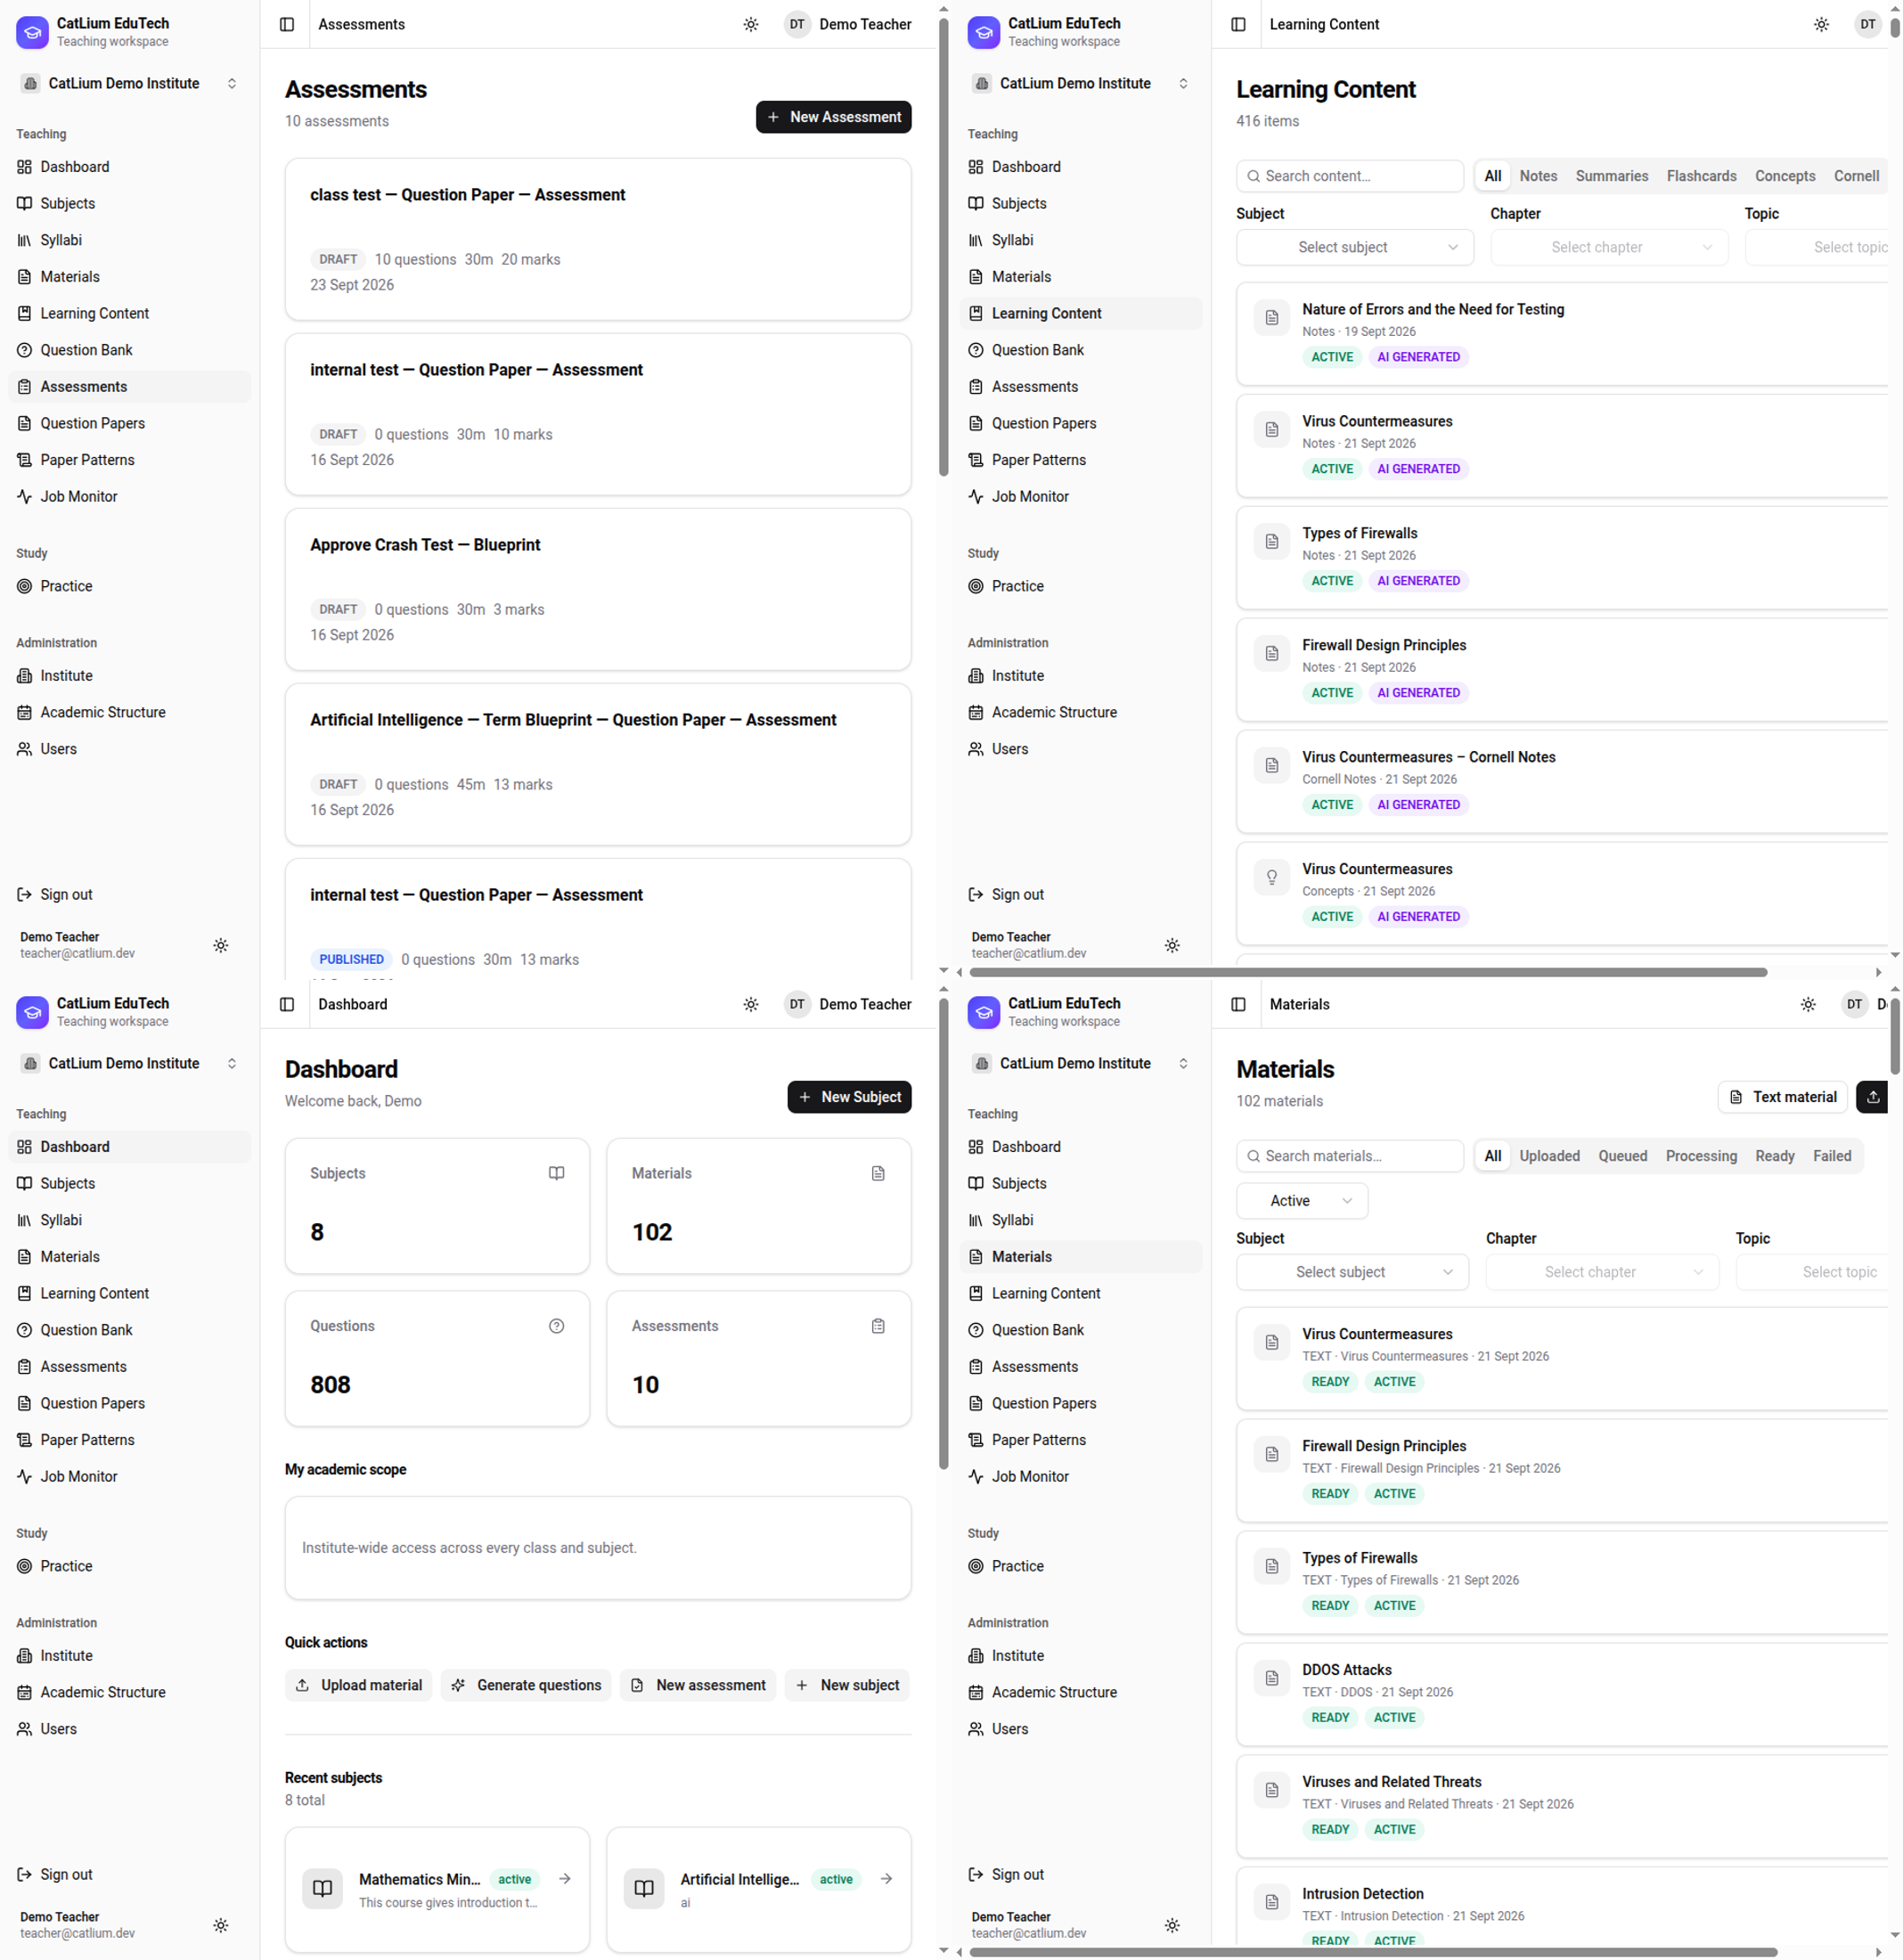
\includegraphics[width=\textwidth,height=\textheight,keepaspectratio]{figures/plate-1.png}
\caption{Plate 1 --- teacher workspace: dashboard, subjects, materials, and
learning content (colour; four per page).}
\label{fig:plate-screenshots-1}
\end{figure}

\begin{figure}[p]
\centering
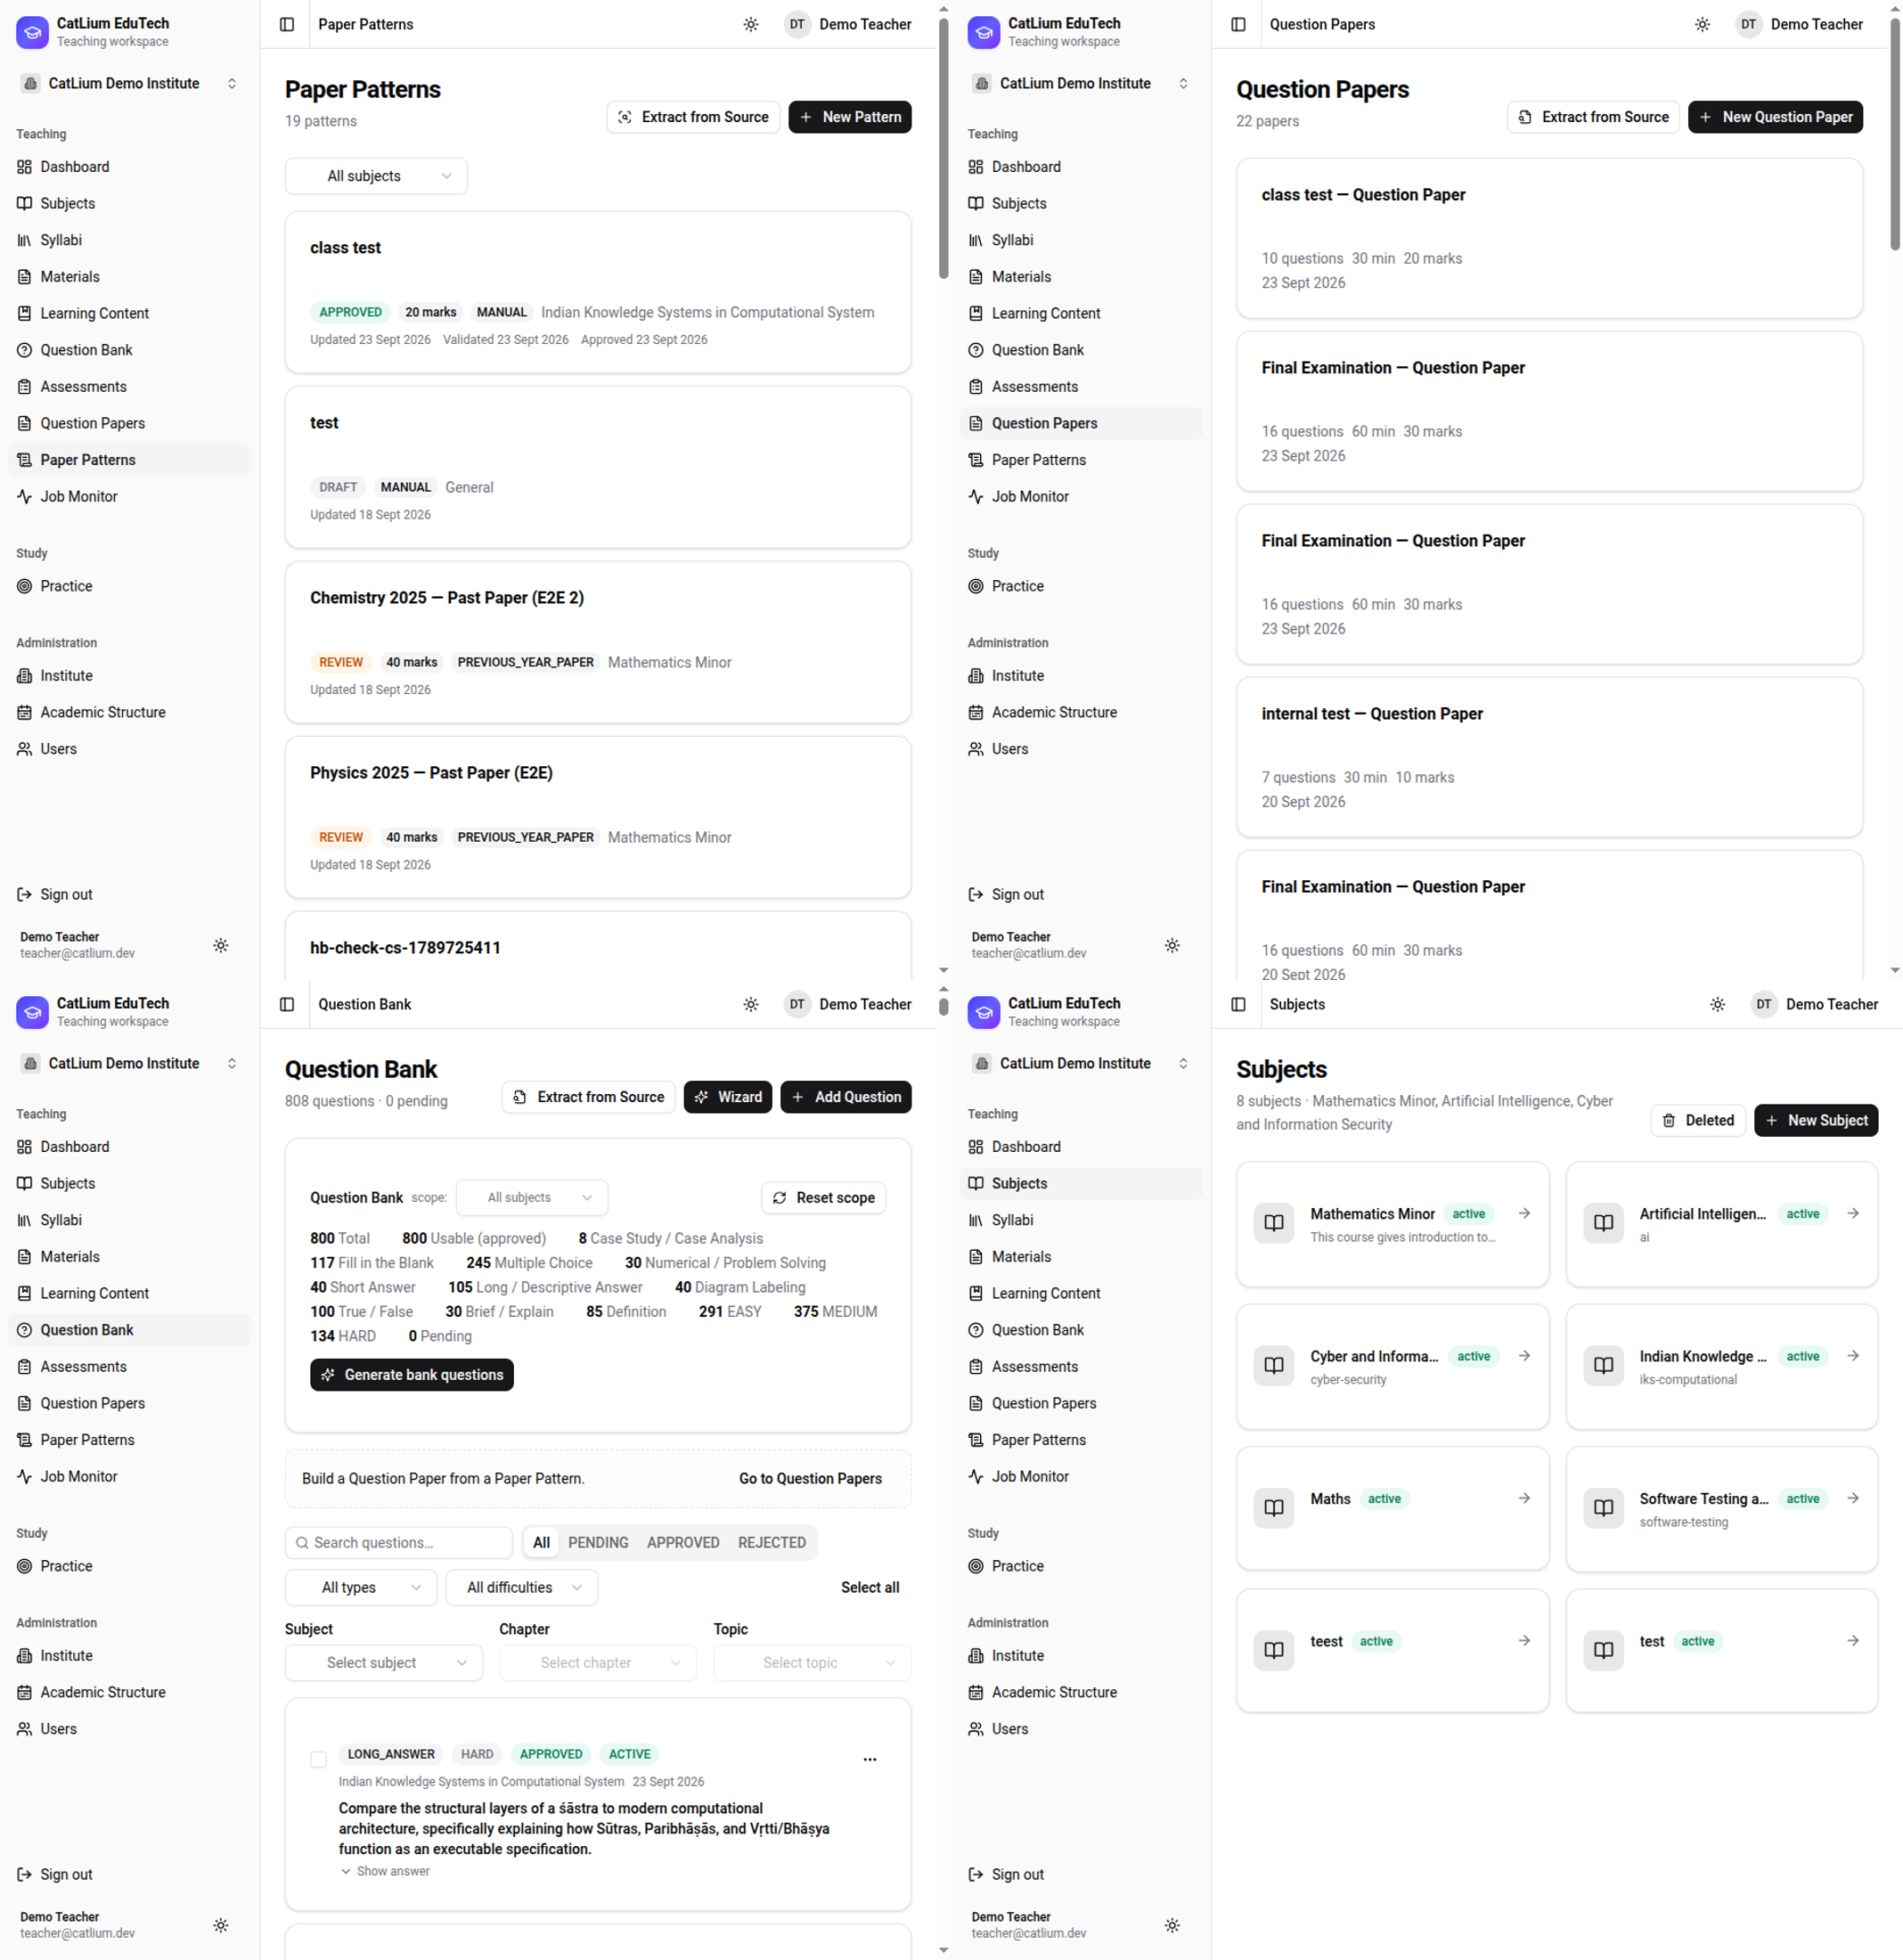
\includegraphics[width=\textwidth,height=\textheight,keepaspectratio]{figures/plate-2.png}
\caption{Plate 2 --- teacher workspace: question bank, question papers, paper
patterns, and assessments (colour; four per page).}
\label{fig:plate-screenshots-2}
\end{figure}
